\renewcommand{\theequation}{\theenumi}
\begin{enumerate}[label=\thesection.\arabic*.,ref=\thesection.\theenumi]
\numberwithin{equation}{enumi}



































%Choose a correct answer\\
















%Choose the correct answer in each of the following:\\











%In each of the following, choose the correct answer:\\















% Choose the correct answer in each of the following:

%\item Which of the following experiments have equally likely outcomes? Explain.
% (i) A driver attempts to start a car. The car starts or does not start.\\
% (ii) A player attempts to shoot a basketball. She/he shoots or misses the shot.\\
% (iii) A trial is made to answer a true-false question. The answer is right or wrong.\\
% (iv) A baby is born. It is a boy or a girl.\\
% \item Why is tossing a coin considered to be a fair way of deciding which team should get the
%ball at the beginning of a football game?





%\item Suppose you drop a die at random on the rectangular region shown in Fig. \ref{fig:1.2.131}. What is the probability that it will land inside the circle with diameter 1m?
%\begin{figure}[!ht]
%\centering
%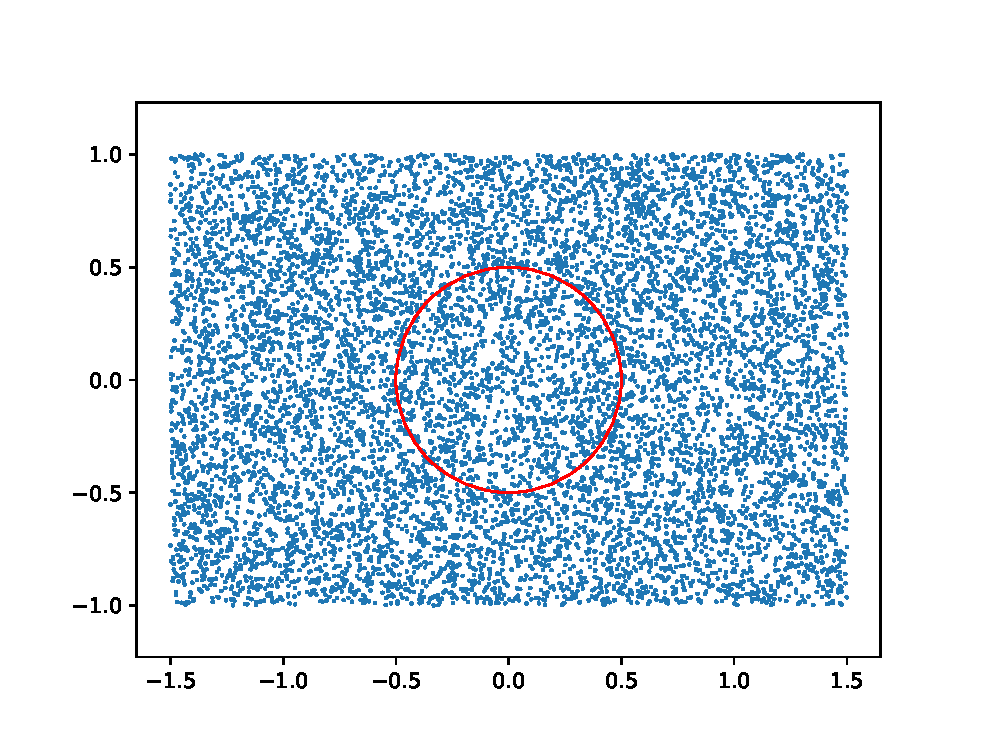
\includegraphics[width=\columnwidth]{./prob/figs/rectangle.eps}
%\caption{}
%\label{fig:1.2.131}
%\end{figure}
%\\
%\solution
%Let X be the random variable representing the number of defective eggs from the ten eggs picked. X follows a  binomial distribution.  Since the probability of an egg being defective is 10\%, substituting n=10, p= 0.1 and k=0 in equation \eqref{eq:exam41_1}, 
probability that there is atleast one defective egg is 
\begin{align}
\pr{X \geq 1}&= 1 - \pr{X=0}  = 1-\brak{0.9}^{10}
\\
&=0.6513215599
\end{align}
The python code for the above problem is,
\begin{lstlisting}
.solutions/20-10/prob/codes/exam42.py
\end{lstlisting}

%\begin{table}[!ht]
%\centering
%\resizebox{\columnwidth}{!}{%
%\begin{tabular}{|c|c|c|c|c|c|c|c|c|c|c|c|}
%\hline
%Event:
%'Sum on 2 dice'&2&3&4&5&6&7&8&9&10&11&12\\
%\hline
%Probability&$\frac{1}{36}$ &-&-&-&-&-& $\frac{5}{36}$ &-&-&-& $\frac{1}{36}$\\
%\hline
%\end{tabular}
%}
%\caption{}
%\label{table:1.2.133}
%\end{table}
%\solution
%Let X be the random variable representing the number of defective eggs from the ten eggs picked. X follows a  binomial distribution.  Since the probability of an egg being defective is 10\%, substituting n=10, p= 0.1 and k=0 in equation \eqref{eq:exam41_1}, 
probability that there is atleast one defective egg is 
\begin{align}
\pr{X \geq 1}&= 1 - \pr{X=0}  = 1-\brak{0.9}^{10}
\\
&=0.6513215599
\end{align}
The python code for the above problem is,
\begin{lstlisting}
.solutions/20-10/prob/codes/exam42.py
\end{lstlisting}


    \end{enumerate}
%\end{document}
    
